\section{Verteilte Systeme in der Service-Oriented Architecture}

In der \emph{Service-Oriented Architecture} (SOA) werden Softwareressourcen als Services verpackt, die eigenständige Module darstellen. Diese bieten standardisierte Geschäftsfunktionalitäten und sind unabhängig vom Zustand oder Kontext anderer Dienste. Es wird eine Sammlung von Services erstellt, die miteinander kommunizieren können, indem eine API verwendet wird, um Nachrichten von einem Service an ein anderes zu übermitteln oder eine Aktivität zwischen zwei oder mehreren Teilen des Systems zu koordinieren. In der Abbildung \ref{fig:serviceOrientatedArchitecture} ist ein einfacher Aufbau mit den Abhängigkeiten der einzelnen Module eines SOAs zu erkennen. Auf diese Weise kann mit SOA ein sehr flexibles, entkoppeltes System geschaffen werden. Jedoch ist die Koordination der Services eine große Herausforderung. Dadurch sind einige Kommunikationstechniken entstanden, welche später im Kapitel \ref{kommunikationstechnikenInVerteilteSysteme} beschrieben werden. Des Weiteren weisen verteilte Systeme gewisse Eigenschaften und Merkmale auf, mithilfe denen eine Bewertung des Systems durchgeführt werden kann. Diese werden nun im Kapitel \ref{eigenschaftenVonVerteiltenSystemen} erläutert.
\cite{papazoglouServiceOrientedArchitectures2007}

\begin{figure}
    \centering
    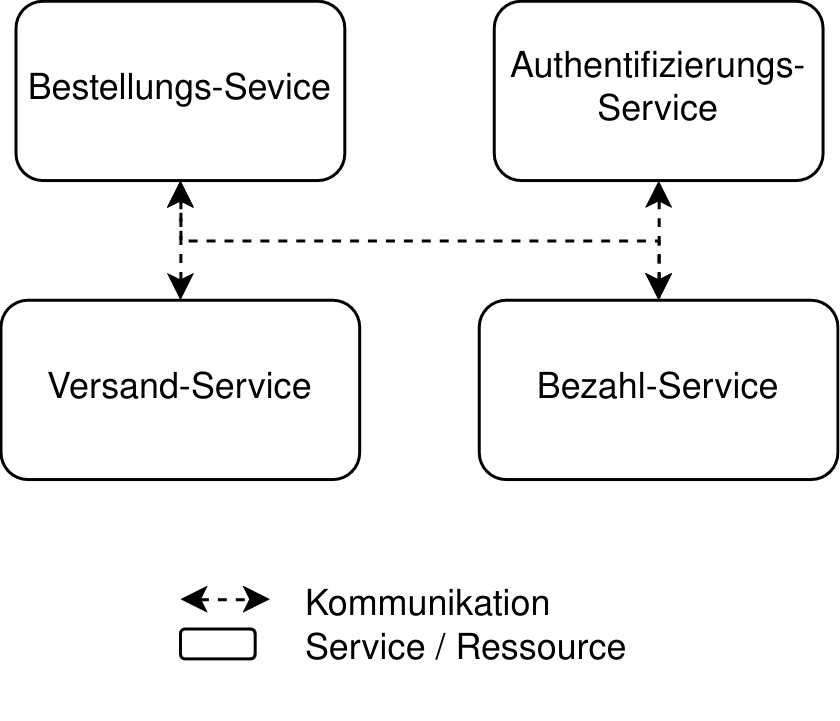
\includegraphics[width=0.6\textwidth]{content/img/Research/Message_Services/serviceOrientatedArchitecture.png}
    \caption{Darstellung eines Systems, welches auf einer Service-Oriented Architecture beruht}
    \label{fig:serviceOrientatedArchitecture}
\end{figure}
\FloatBarrier

\subsection{Eigenschaften zur Bewertung von verteilten Systeme}
\label{eigenschaftenVonVerteiltenSystemen}
Die Entwicklung eines verteilten Systems ist kein leichtes Unterfangen. Dadurch ist es sehr wichtig, die Funktionsfähigkeit des Anwendungssystems ermitteln zu können. In der folgenden Liste sind die Eigenschaften und Merkmale eines SOA-Systems aufgezählt, welche eine leichte Bewertung ermöglichen. \cite{toshevLearningRabbitMQBuild2016,curryMessageOrientedMiddleware2004}

\begin{itemize}
	\item \textbf{Kopplung}: Eine hohe Entkopplung der einzelnen Komponenten spielt eine wichtige Rolle, um eine unabhängige Entwicklung und eine hohe Flexibilität der Anwendung zu erreichen.
	\item \textbf{Latenz}: Da in verteilten Systemen die Ressourcen aufgeteilt werden, ist es von Bedeutung, die Kommunikation der Komponenten mit einer niedrigen Verzögerung zu gewährleisten.
	\item \textbf{Skalierbarkeit}: Moderne Anwendungen müssen in der Lage sein, sich an die Belastung anzupassen, die durch die Interaktion der Benutzer mit der Software entsteht. Dies ermöglicht einen reibungslosen, nicht frustrierenden Ablauf für die Benutzer.
	\item \textbf{Wartbarkeit}: Verteilte Systeme müssen in der Lage sein, ihre Komplexität zu abstrahieren und dadurch eine leichte Wartbarkeit zu realisieren. Denn nicht überschaubare Systeme stellen langfristig einen erheblichen Kostenfaktor in der Entwicklung und Wartung dar.
	\item \textbf{Zuverlässigkeit}: Um eine erfolgreiche Anwendung zu gewährleisten, bedarf es einer Software mit hoher Robustheit und Zuverlässigkeit, da Fehler in der Anwendung unerwünschte Auswirkungen haben können, die in Produktivsystemen nicht toleriert werden können.
	\item \textbf{Verfügbarkeit}: Wenn es zu Ausfällen von Anwendungssystemen kommt, können erhebliche Kosten in Millionenhöhe entstehen. Daher ist es von entscheidender Relevanz, diese Ausfälle zu minimieren und eine stetige Verfügbarkeit zu gewährleisten.
	\item \textbf{Erweiterbarkeit}: Im Lebenszyklus einer Anwendung ist die kontinuierliche Erweiterbarkeit tief verankert, da sich Geschäftsszenarien ständig ändern können. Eine Software, die die Fähigkeit besitzt, sich flexibel an diese Anforderungen anzupassen, bietet erhebliche Vorteile.
\end{itemize}

\subsection{Kommunikationstechniken in verteilte Systeme}
\label{kommunikationstechnikenInVerteilteSysteme}

Die Koordination und Kommunikation in verteilten Systemen können schnell zu einer äußerst anspruchsvollen Aufgabe werden, sobald das System eine bestimmte Größe erreicht. Die Synchronisation und Koordination von Services im Allgemeinen bei solchen Systemen ist nicht trivial. Beispielsweise müssen Sie sich nur einmal vorstellen, aus wie vielen kleinen Services alle Google Apps bestehen müssen, damit Millionen von Nutzern gleichzeitig damit arbeiten können. Es ist offensichtlich, dass solche Systeme leicht zu einem unüberschaubaren Netzwerk von Abhängigkeiten werden können. Ein weiterer Punkt, welcher zu beachten ist, wäre: Was passiert, wenn ein Service ausfällt und damit der Zugriff auf eine Ressource nicht mehr möglich ist? Eine Ausnahmesituation dieser Art kann leicht zu Inkonsistenzen im System führen oder im Extremfall eine Kettenreaktion auslösen, die zu einem totalen Ausfall der gesamten Anwendung führt. Damit solche Szenarien vermieden werden können und der Informationsaustausch der Module des verteilten Systems verlässlich und einfach gestaltet werden kann, haben sich verschiedene Kommunikationstechniken etabliert, welche in den nachfolgenden Unterkapiteln erklärt und verglichen werden. \cite{google2009services}

\subsubsection{Direkte Kommunikation zwischen den Services}

Die trivialste Lösung wäre eine Form von \emph{Remote Procedure Calls (RPC)} zwischen den einzelnen Teilen des verteilten Systems. Ein RPC ist eine Technik, die es einem Programm ermöglicht, eine Funktion oder Methode in einem anderen entfernten Programm aufzurufen, als ob sie lokal aufgerufen würde. Allerdings führt dies zu einer hohen Kopplung, da die einzelnen Services direkt miteinander kommunizieren, wie es in der Darstellung \ref{fig:direkteKommunikationMOM} zu erkennen ist. 
Die Natur dieser Kommunikationstechnik benötigt eine synchrone Übertragung, weil die Kommunikationspartner stets auf die Rückmeldung des anderen warten müssen, um Gewissheit zu erlangen, dass die Nachricht erfolgreich übermittelt wurde. Die synchrone Übertragung hat eine geringere Skalierbarkeit im Gegensatz zur asynchronen Übertragung, da durch das Warten auf die Rückmeldung Verzögerungen entstehen.    
Wenn diese Systeme eine gewisse Größe erreichen, werden sie zu undurchsichtigen Netzen an Abhängigkeiten, was zu aufwendiger Wartung und erschwerter Erweiterung des Systems führt. Dennoch können die Anforderungen an die Echtzeitkommunikation erfüllt werden, da alle Services direkt miteinander kommunizieren.
\cite{toshevLearningRabbitMQBuild2016,curryMessageOrientedMiddleware2004}

\begin{figure}
    \centering
    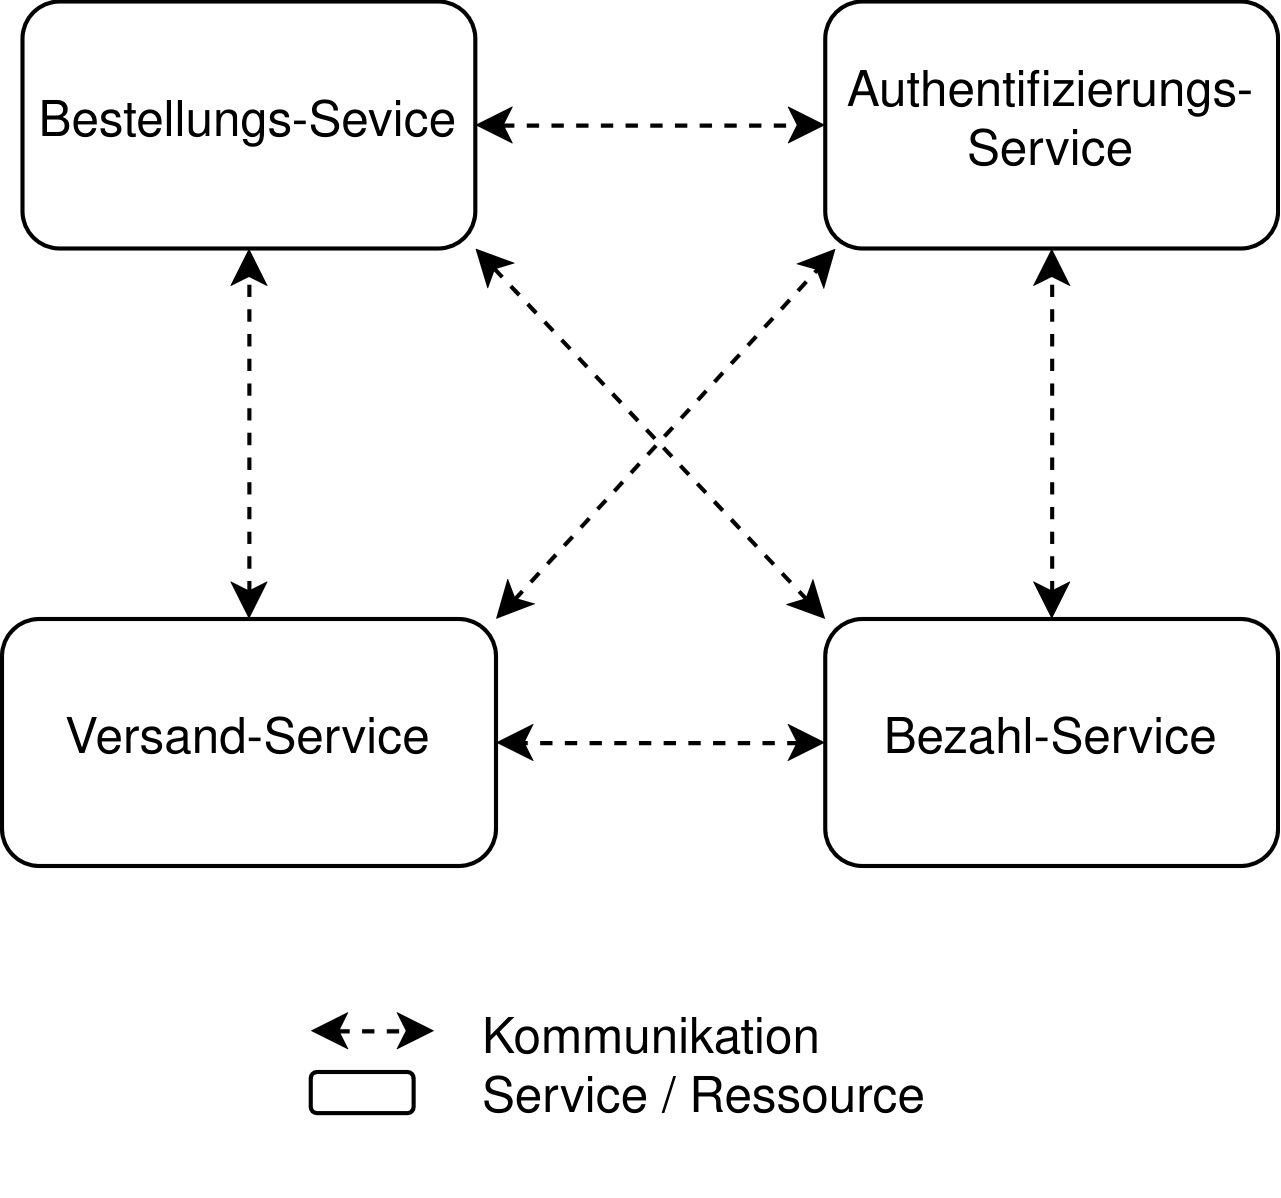
\includegraphics[width=0.6\textwidth]{content/img/Research/Message_Services/direktKommunikationMOM.png}
    \caption{Ein Beispiel für ein verteiltes System mit direkter Kommunikation \cite{curryMessageOrientedMiddleware2004}}
    \label{fig:direkteKommunikationMOM}
\end{figure}
\FloatBarrier

\subsubsection{Verwendung einer gemeinsamen Datenbank}

Eine weitere Möglichkeit des Informationsaustauschs könnte die Kommunikation über eine gemeinsame Datenbank sein. In dieser Architektur sind alle Services von dem gleichen Datenbank-Schema abhängig, welches die Koppelung reduziert. Durch die Zentralisierung der Kommunikationswege, wie es in der Abbildung \ref{fig:datenbankKommunikationRabbit} erkennbar ist, wird ein sehr übersichtlicher Aufbau des verteilten Systems geschaffen. Weitere Services können auch leicht integriert werden, da sie nur mit dem Datenbank-Schema kommunizieren müssen. Wenn jedoch das Datenbank-Schema angepasst wird, müssen alle Module angepasst werden. Dieser Prozess könnte mit großem Aufwand verbunden sein. Eine hohe Skalierbarkeit zu erreichen, ist in den meisten Fällen sehr herausfordernd, da jedes Modul den zentralen Punkt belastet, insbesondere bei relationalen Datenbanken, da diese von Natur aus schwer zu skalieren sind. \cite{toshevLearningRabbitMQBuild2016,curryMessageOrientedMiddleware2004}

\begin{figure}
    \centering
    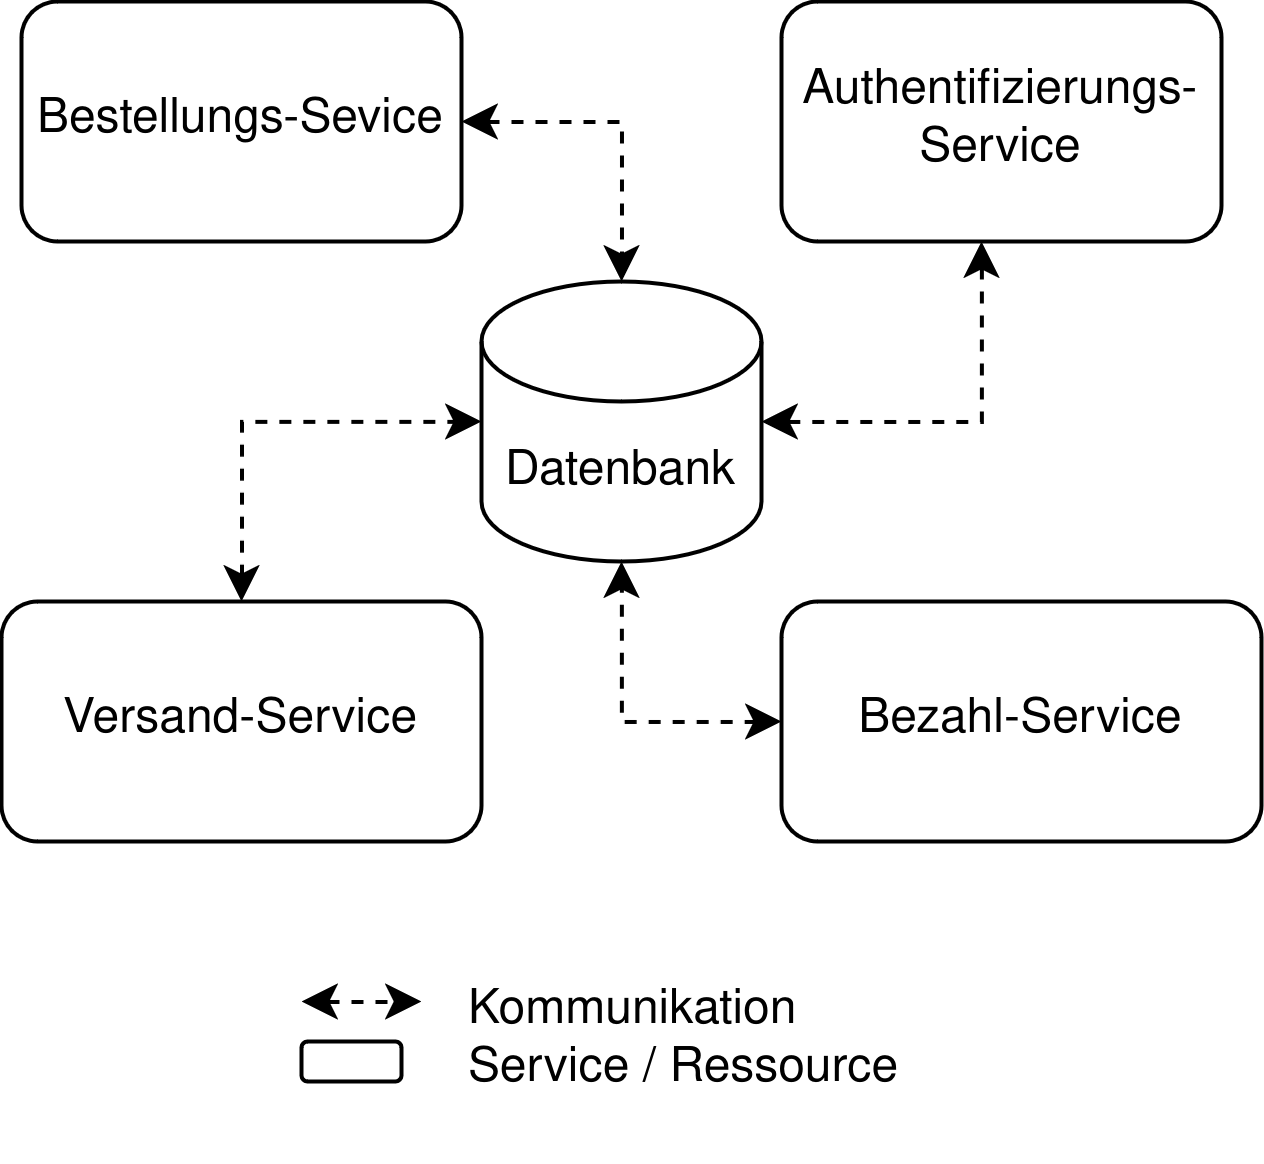
\includegraphics[width=0.6\textwidth]{content/img/Research/Message_Services/datenbankKommunikationRabbit.png}
    \caption{System mit Datenbank als zentraler Kommunikationskomponente}
    \label{fig:datenbankKommunikationRabbit}
\end{figure}
\FloatBarrier

\subsubsection{Nutzung von einem Messaging System}

Bei der Verwendung von einem oder mehreren Messaging Systemen wird jegliche Kommunikation über einen oder mehrere zentrale Punkte geleitet, wie in der Abbildung \ref{fig:messagingSystemsKommunikation} zu erkennen ist. Ein Sender schickt seine Nachricht zu dem Nachrichten-System, welches die Information an einen oder mehrere Empfängern weiterleitet. \cite{curryMessageOrientedMiddleware2004}

Durch den zentralisierten Aufbau bleibt das verteilte System übersichtlich und wartbar, was beim Auftreten eines Fehlers zu einer erheblich vereinfachten Ursprungssuche führt.
Die Kopplung der Services ist sehr niedrig, weil das Messaging-System eine zusätzliche Schicht zwischen dem Empfänger und dem Sender vertritt. Somit können auch beispielsweise alte Services leicht mit moderneren ersetzt werden. \cite{toshevLearningRabbitMQBuild2016}

Die Übertragung ist in diesem Fall vollständig asynchron, da die Kommunikationspartner nicht auf die Antwort des anderen warten müssen, weil die Nachricht einfach an einen Vermittler übergeben wird. Die Skalierbarkeit von verteilten Systemen, welche Messaging Systeme verwenden, ist aufgrund deren asynchronen Natur grundsätzlich sehr hoch und kann daher auch zu Spitzenzeiten die Last der Benutzer standhalten. \cite{toshevLearningRabbitMQBuild2016}

Zusätzlich wird auch die zuverlässige Nachrichtenübertragung sichergestellt. Dies rüht daher, weil Nachrichten, die nicht zugestellt werden können, da der Empfänger momentan nicht erreichbar ist, zwischengespeichert werden, damit diese zu einem späteren Zeitpunkt an den Empfänger gesendet werden können. \cite{curryMessageOrientedMiddleware2004}

Des Weiteren ermöglicht eine Architektur mit Messaging-Systemen eine einfache Erweiterbarkeit. Denn durch das Hinzufügen eines weiteren Services werden keine bestehenden Kommunikationskanäle beeinträchtigt. Somit kann das System mittels neuen Komponenten ohne großen Aufwand um dessen Funktionalität erweitert werden. Dies trägt dazu bei, dass das System flexibel bleibt und mit den Anforderungen des Unternehmens oder der Anwendung mitwachsen kann. \cite{curryMessageOrientedMiddleware2004}

In Bezug auf die Latenz bietet die Verwendung von Messaging-Systemen oft niedrige Verzögerungszeiten, insbesondere aufgrund der asynchronen Übertragung. Dies ermöglicht eine effiziente und zeitnahe Kommunikation zwischen den verschiedenen Komponenten eines verteilten Systems. \cite{curryMessageOrientedMiddleware2004}

\begin{figure}
    \centering
    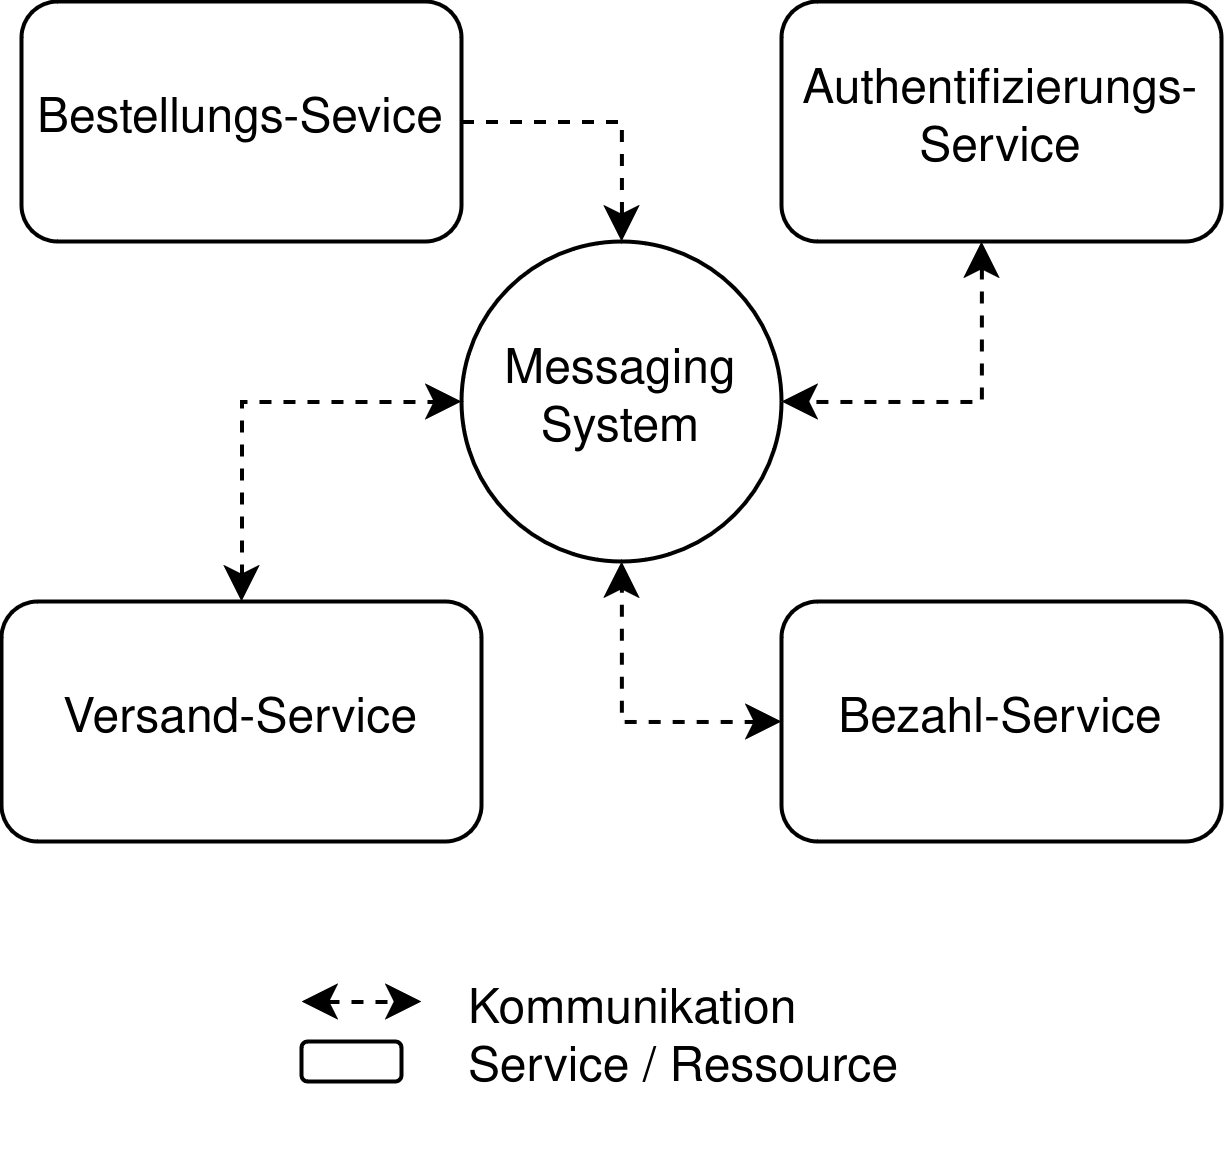
\includegraphics[width=0.6\textwidth]{content/img/Research/Message_Services/kommunikationWithMessagingSystemRabbitMQ.png}
    \caption{Messaging System als zentraler Kommunikationsknoten}
    \label{fig:messagingSystemsKommunikation}
\end{figure}
\FloatBarrier

Im folgenden Kapitel werden wir nun detailliert auf die Funktionsweise eines EMS eingehen.
